\documentclass[12pt, a4paper]{article}
\usepackage[a4paper, margin=3cm]{geometry}
\usepackage{graphicx}
\usepackage{setspace}
% \usepackage{times}
\usepackage{ragged2e}
\usepackage{graphicx}
\usepackage{titling}
\usepackage{geometry}
\usepackage{listings}
\usepackage{xcolor}
\usepackage{float}
\usepackage{hyperref}
\usepackage{indentfirst}
\usepackage{setspace}
% \usepackage[natbibapa]{apacite}
% \usepackage{natbib}
\usepackage{chngcntr}
\usepackage{amsmath}
\usepackage{amssymb}

\renewcommand{\figurename}{Gambar}
\renewcommand\thesection{\Alph{section}}

\definecolor{codebg}{RGB}{255,255,255}   % background putih seperti sel Jupyter
\definecolor{codetext}{RGB}{0,0,0}
\definecolor{linenumcol}{RGB}{128,128,128}
\definecolor{pykw}{RGB}{0,128,0}         % keyword (def, if, for, import, dll) - hijau
\definecolor{pystr}{RGB}{186,33,33}      % string - merah kecoklatan
\definecolor{commentcol}{RGB}{64,128,128}% comment - abu kebiruan
\definecolor{pyfunc}{RGB}{0,0,255}       % fungsi/built-in - biru
\definecolor{pyconst}{RGB}{0,128,0}      % True/False/None - hijau (sama seperti keyword)
\definecolor{pyvar}{RGB}{150,0,150}      % variabel khusus (opsional)

\lstdefinestyle{pythonnb}{
    backgroundcolor=\color{codebg},
    basicstyle=\ttfamily\small\color{codetext},
    breaklines=true,
    breakatwhitespace=true,
    tabsize=4,
    showstringspaces=false,
    numbers=left,
    numberstyle=\tiny\color{linenumcol},
    numbersep=10pt,
    frame=single,
    rulecolor=\color{gray!40},
    framesep=5pt,
    xleftmargin=18pt,
    % Bahasa Python
    language=Python,
    morekeywords={self, as, with, lambda, yield, async, await},
    keywordstyle=\color{pykw}\bfseries,
    % String (merah kecoklatan)
    stringstyle=\color{pystr},
    % Comment (abu kebiruan, italic)
    commentstyle=\color{commentcol}\itshape,
    % Fungsi / built-in umum (biru)
    emph={print, len, range, int, str, float, type, open, input, list, dict, set, tuple, sum, min, max, sorted, enumerate, zip, map, filter, isinstance},
    emphstyle=\color{pyfunc},
    % Konstanta True/False/None (hijau, bold)
    emph={[2]True, False, None},
    emphstyle={[2]\color{pyconst}\bfseries},
}
\usepackage{chngcntr}

\begin{document}



\begin{titlepage}
    \centering
    \onehalfspacing
    
    % Judul
    { \textbf{LAPORAN PRAKTIKUM}}\\[0.3cm]
    { \textbf{PRAKTIKUM PENAMBANGAN DATA}}\\[0.3cm]
    { \textbf{PERTEMUAN 4}}\\[0.3cm]
    { \textbf{REGRESI}} \\[1.5cm]
    
    % Logo (ganti ugm.png dengan nama file logo kamu)
    \includegraphics[height=7cm]{../images/ugm.png}
    
    % Identitas
    \begin{center}
Disusun oleh:\\[0.3cm]
\end{center}

\begin{center}
    \begin{tabular}{l c l}
        Nama & : & Hanan Fijananto \\
        NIM & : & 24/538946/SV/24555 \\
        Kelas & : & A2\\ 
        Dosen Pengampu & : & Dr.Imam Fahrurrozi, S.T., M.Cs.
    \end{tabular}
\end{center}


    
    \vspace{1.5cm}
    
    % Footer bawah
    { \textbf{PROGRAM STUDI D-IV TEKNOLOGI REKAYASA PERANGKAT LUNAK}}\\[0.3cm]
    { \textbf{DEPARTEMEN TEKNIK ELEKTRO DAN INFORMATIKA}}\\[0.3cm]
    { \textbf{SEKOLAH VOKASI}}\\[0.3cm]
    { \textbf{UNIVERSITAS GADJAH MADA}}\\[0.3cm]
    { \textbf{YOGYAKARTA}}\\[0.3cm]
    {\textbf{2026}}
    
\end{titlepage}

\doublespacing 

\section{Tujuan}
\begin{enumerate}
    \item Mahasiswa mampu memahami konsep dasar regresi dan algoritma regresi.
    \item Mahasiswa mengetahui prinsip kerja berbagai algoritma regresi, khususnya Linear 
Regression, Decision Tree Regression, dan Random Forest Regression 
    \item Mahasiswa mampu melakukan evaluasi model regresi menggunakan metrik RMSE dan $R^2$.
    \item  Mahasiswa dapat menerapkan berbagai algoritma regresi untuk membangun model.
\end{enumerate}
\section{Dasar Teori}
\subsection{Regresi}
Regresi merupakan salah satu metode dalam pembelajaran mesin dan statistika yang digunakan untuk memodelkan hubungan antara variabel independen atau variabel prediktor dengan variabel dependen atau variabel target yang memiliki nilai kontinu. Tujuan utama regresi adalah menghasilkan suatu model yang dapat digunakan untuk memperkirakan nilai variabel target berdasarkan informasi yang terdapat pada variabel prediktor. Dalam konteks pembelajaran mesin, model regresi dibangun menggunakan data pelatihan untuk mempelajari pola hubungan antara fitur masukan dan nilai target, kemudian digunakan untuk melakukan prediksi terhadap data baru.

Secara umum, permasalahan regresi dapat dinyatakan sebagai pasangan data $(x_i,y_i)$, dengan $x_i$ merupakan vektor fitur pada pengamatan ke-$i$ dan $y_i$ merupakan nilai target yang ingin diprediksi. Model regresi berusaha menemukan suatu fungsi $\hat{f}$ sehingga nilai prediksi $\hat{y}_i = \hat{f}(x_i)$ memiliki kedekatan dengan nilai aktual $y_i$. Salah satu tujuan utama proses pembelajaran tersebut adalah meminimalkan kesalahan antara nilai aktual dan nilai hasil prediksi \cite{james2021statistical}.

Regresi berbeda dengan klasifikasi. Pada klasifikasi, variabel target berupa kategori atau kelas, sedangkan pada regresi variabel target umumnya berupa nilai numerik kontinu. Oleh karena itu, regresi dapat digunakan pada permasalahan seperti prediksi harga, jumlah permintaan, pendapatan, suhu, konsumsi energi, dan berbagai variabel numerik lainnya.

\subsection{Algoritma Regresi}

Algoritma regresi merupakan metode atau pendekatan yang digunakan untuk membentuk fungsi prediksi berdasarkan data yang tersedia. Algoritma tersebut mempelajari pola hubungan antara variabel prediktor dan variabel target melalui proses pelatihan. Setelah model terbentuk, model dapat digunakan untuk menghasilkan prediksi terhadap data yang belum pernah digunakan dalam proses pelatihan.

Terdapat berbagai algoritma yang dapat digunakan untuk menyelesaikan permasalahan regresi. Pemilihan algoritma bergantung pada karakteristik data, hubungan antara variabel, kompleksitas pola, serta kebutuhan interpretasi model. Beberapa algoritma yang umum digunakan antara lain Linear Regression, Decision Tree Regression, Random Forest Regression, Support Vector Regression, dan berbagai algoritma berbasis ensemble lainnya \cite{james2021statistical}.

Dalam penelitian ini, algoritma regresi yang digunakan adalah Linear Regression, Decision Tree Regression, dan Random Forest Regression. Ketiga algoritma tersebut memiliki pendekatan yang berbeda dalam memodelkan hubungan antara variabel prediktor dan variabel target.

\subsection{Linear Regression}

Linear Regression atau regresi linear merupakan salah satu metode regresi yang digunakan untuk memodelkan hubungan linear antara variabel prediktor dengan variabel target. Metode ini mengasumsikan bahwa perubahan pada variabel target dapat dijelaskan melalui kombinasi linear dari variabel prediktor.

Pada regresi linear dengan satu variabel prediktor, bentuk umum model dapat dituliskan sebagai:

\begin{equation}
\hat{y} = \beta_0 + \beta_1x
\end{equation}

dengan $\hat{y}$ merupakan nilai prediksi, $\beta_0$ merupakan intercept atau konstanta, $\beta_1$ merupakan koefisien regresi, dan $x$ merupakan variabel prediktor. Pada regresi linear berganda yang menggunakan lebih dari satu variabel prediktor, persamaan dapat dituliskan sebagai:

\begin{equation}
\hat{y} = \beta_0 + \beta_1x_1 + \beta_2x_2 + \cdots + \beta_px_p
\end{equation}

Koefisien regresi diperoleh melalui proses estimasi yang bertujuan menemukan parameter model sehingga nilai prediksi memiliki kesalahan sekecil mungkin terhadap nilai aktual. Salah satu pendekatan yang umum digunakan adalah Ordinary Least Squares (OLS), yaitu dengan meminimalkan jumlah kuadrat residual antara nilai aktual dan nilai prediksi \cite{james2021statistical}.

\begin{equation}
\underset{\beta}{\operatorname{minimize}}
\sum_{i=1}^{n}(y_i-\hat{y}_i)^2
\end{equation}

Residual merupakan selisih antara nilai aktual dengan nilai prediksi yang dapat dirumuskan sebagai:

\begin{equation}
e_i = y_i-\hat{y}_i
\end{equation}

Implementasi Linear Regression pada \textit{Scikit-learn} menyediakan estimator \texttt{LinearRegression} yang digunakan untuk melakukan prediksi berdasarkan model linear. Evaluasi model regresi tersebut juga dapat dilakukan menggunakan koefisien determinasi $R^2$ \cite{scikitLearnLinearRegression}.

\subsection{Decision Tree Regression}

Decision Tree Regression merupakan metode regresi berbasis pohon keputusan yang membagi ruang data menjadi beberapa bagian berdasarkan aturan pemisahan tertentu. Berbeda dengan Linear Regression yang membentuk hubungan linear, Decision Tree Regression dapat memodelkan hubungan yang tidak linear antara variabel prediktor dan variabel target.

Proses pembentukan Decision Tree Regression dilakukan dengan melakukan pemisahan data secara bertahap berdasarkan fitur dan nilai ambang tertentu. Setiap pemisahan menghasilkan beberapa subset data yang kemudian dapat kembali dipisahkan hingga memenuhi kondisi penghentian tertentu. Pada bagian akhir pohon terdapat \textit{leaf} atau simpul terminal yang digunakan untuk menghasilkan nilai prediksi.

Pada permasalahan regresi, salah satu kriteria yang dapat digunakan untuk menentukan kualitas pemisahan adalah Mean Squared Error (MSE). Untuk suatu node $m$ yang memiliki $n_m$ observasi, MSE dapat dinyatakan sebagai:

\begin{equation}
MSE_m =
\frac{1}{n_m}
\sum_{y_i \in Q_m}
(y_i-\bar{y}_m)^2
\end{equation}

dengan $Q_m$ merupakan kumpulan data yang berada pada node $m$ dan $\bar{y}_m$ merupakan nilai rata-rata target pada node tersebut. Pemisahan dipilih berdasarkan pengurangan kesalahan yang dihasilkan oleh pembagian data. Pada simpul terminal, nilai prediksi umumnya berupa rata-rata nilai target dari data yang berada pada simpul tersebut ketika menggunakan kriteria squared error \cite{scikitLearnDecisionTree}.

Decision Tree Regression memiliki kemampuan untuk menangkap hubungan non-linear dan interaksi antarvariabel tanpa memerlukan transformasi matematis tertentu. Namun, pohon keputusan yang terlalu kompleks dapat mengalami \textit{overfitting}, yaitu kondisi ketika model sangat baik dalam memprediksi data pelatihan tetapi memiliki kemampuan generalisasi yang rendah terhadap data baru.

\subsection{Random Forest Regression}

Random Forest Regression merupakan algoritma ensemble yang menggabungkan sejumlah Decision Tree untuk menghasilkan prediksi yang lebih stabil dan umumnya memiliki kemampuan generalisasi yang lebih baik dibandingkan sebuah pohon keputusan tunggal. Konsep Random Forest diperkenalkan oleh Breiman sebagai kumpulan prediktor berbasis pohon yang masing-masing dibangun menggunakan unsur pengacakan tertentu \cite{breiman2001random}.

Dalam Random Forest Regression, beberapa pohon keputusan dibangun menggunakan variasi data pelatihan dan pemilihan fitur secara acak. Setiap pohon menghasilkan prediksi terhadap suatu observasi, kemudian hasil prediksi dari seluruh pohon digabungkan. Untuk permasalahan regresi, penggabungan tersebut umumnya dilakukan dengan menghitung rata-rata prediksi dari seluruh pohon.

Jika terdapat $B$ pohon keputusan dan prediksi dari pohon ke-$b$ adalah $\hat{f}_b(x)$, maka prediksi Random Forest dapat dinyatakan sebagai:

\begin{equation}
\hat{f}_{RF}(x)
\frac{1}{B}
\sum_{b=1}^{B}\hat{f}_b(x)
\end{equation}

Penggunaan banyak pohon dengan variasi data dan fitur dapat mengurangi ketergantungan model terhadap satu struktur pohon tertentu. Random Forest juga dapat digunakan untuk memperkirakan pentingnya variabel dalam proses prediksi. Menurut Breiman, pendekatan Random Forest dapat digunakan baik untuk permasalahan klasifikasi maupun regresi \cite{breiman2001random}.

Meskipun demikian, Random Forest memiliki kompleksitas yang lebih tinggi dibandingkan Linear Regression. Model juga cenderung lebih sulit diinterpretasikan karena hasil prediksi berasal dari kombinasi banyak pohon keputusan. Oleh karena itu, pemilihan Random Forest perlu mempertimbangkan kebutuhan antara kemampuan prediksi, kompleksitas model, dan interpretabilitas.

\subsection{Metrik Evaluasi Regresi}

Metrik evaluasi regresi digunakan untuk mengukur seberapa baik model menghasilkan prediksi terhadap nilai aktual. Evaluasi diperlukan karena nilai prediksi yang dihasilkan model belum dapat menunjukkan kualitas model tanpa dibandingkan dengan nilai sebenarnya.

Beberapa metrik yang umum digunakan dalam evaluasi regresi adalah Mean Absolute Error (MAE), Mean Squared Error (MSE), Root Mean Squared Error (RMSE), Mean Absolute Percentage Error (MAPE), dan Coefficient of Determination ($R^2$). Scikit-learn menyediakan berbagai metrik tersebut sebagai bagian dari evaluasi model regresi \cite{scikitLearnMetrics}.

Dalam penelitian ini, metrik yang digunakan adalah RMSE dan $R^2$. Penggunaan kedua metrik tersebut memungkinkan evaluasi dilakukan dari dua sudut pandang, yaitu besarnya kesalahan prediksi dan kemampuan model dalam menjelaskan variasi nilai target.

\subsection{Root Mean Squared Error (RMSE)}

Root Mean Squared Error (RMSE) merupakan metrik evaluasi yang digunakan untuk mengukur besarnya rata-rata kesalahan prediksi dengan memberikan penalti yang lebih besar terhadap kesalahan yang bernilai besar. RMSE diperoleh dengan menghitung akar kuadrat dari rata-rata kuadrat selisih antara nilai aktual dan nilai prediksi.

RMSE dapat dirumuskan sebagai:

\begin{equation}
RMSE =
\sqrt{
\frac{1}{n}
\sum_{i=1}^{n}
(y_i-\hat{y}_i)^2
}
\end{equation}

dengan $n$ merupakan jumlah observasi, $y_i$ merupakan nilai aktual pada observasi ke-$i$, dan $\hat{y}_i$ merupakan nilai prediksi model.

Nilai RMSE yang semakin kecil menunjukkan bahwa nilai prediksi model semakin dekat dengan nilai aktual. Nilai RMSE sebesar $0$ menunjukkan bahwa seluruh prediksi sama dengan nilai aktual. Karena menggunakan operasi kuadrat, RMSE memberikan pengaruh yang lebih besar terhadap kesalahan prediksi yang besar dibandingkan kesalahan yang kecil. NIST juga menjelaskan akar dari rata-rata kuadrat residual sebagai salah satu ukuran untuk mengevaluasi kualitas kecocokan suatu model, dengan nilai yang lebih kecil menunjukkan kecocokan yang lebih baik \cite{nistGoodnessFit}.

Salah satu kelebihan RMSE adalah satuannya sama dengan variabel target sehingga hasilnya relatif mudah diinterpretasikan. Sebagai contoh, apabila variabel target memiliki satuan rupiah, maka RMSE juga memiliki satuan rupiah.

\subsection{Coefficient of Determination ($R^2$)}

Coefficient of Determination atau koefisien determinasi ($R^2$) merupakan metrik yang digunakan untuk mengukur proporsi variasi pada variabel target yang dapat dijelaskan oleh model berdasarkan variabel prediktor. Dengan demikian, $R^2$ memberikan informasi mengenai seberapa baik model menjelaskan variasi nilai target dibandingkan dengan model sederhana yang hanya menggunakan nilai rata-rata target.

Nilai $R^2$ dapat dirumuskan sebagai:

\begin{equation}
R^2 =
1 -
\frac{
\sum_{i=1}^{n}(y_i-\hat{y}*i)^2
}{
\sum*{i=1}^{n}(y_i-\bar{y})^2
}
\end{equation}

dengan $y_i$ merupakan nilai aktual, $\hat{y}_i$ merupakan nilai prediksi, dan $\bar{y}$ merupakan rata-rata nilai aktual.

Nilai $R^2$ maksimum adalah $1$. Nilai yang semakin mendekati $1$ menunjukkan bahwa model mampu menjelaskan variasi data dengan lebih baik. Nilai $R^2=0$ menunjukkan bahwa model memiliki performa yang setara dengan model sederhana yang selalu memprediksi nilai rata-rata target. Sementara itu, nilai $R^2$ dapat bernilai negatif apabila performa model lebih buruk dibandingkan prediksi menggunakan nilai rata-rata target \cite{scikitLearnMetrics}.

Nilai $R^2$ tidak secara langsung menunjukkan besarnya kesalahan prediksi dalam satuan asli variabel target. Oleh karena itu, penggunaan $R^2$ sebaiknya dipadukan dengan metrik berbasis error seperti RMSE. RMSE memberikan informasi mengenai besar kesalahan prediksi, sedangkan $R^2$ memberikan informasi mengenai kemampuan model dalam menjelaskan variasi data.

\subsection{Perbandingan Algoritma Regresi}

Ketiga algoritma yang digunakan memiliki karakteristik yang berbeda. Linear Regression sesuai digunakan ketika hubungan antara variabel prediktor dan target cenderung linear serta interpretasi koefisien model menjadi salah satu kebutuhan utama. Decision Tree Regression lebih fleksibel dalam menangkap hubungan non-linear, tetapi pohon yang terlalu dalam berpotensi mengalami \textit{overfitting}. Sementara itu, Random Forest Regression menggabungkan banyak Decision Tree sehingga dapat menghasilkan model yang lebih robust terhadap variasi data, tetapi memiliki kompleksitas dan kebutuhan komputasi yang lebih tinggi.

Oleh karena itu, pemilihan model tidak hanya didasarkan pada algoritma yang digunakan, tetapi juga pada hasil evaluasi menggunakan data pengujian. Model dengan nilai RMSE yang lebih rendah dan nilai $R^2$ yang lebih tinggi secara umum menunjukkan performa prediksi yang lebih baik, dengan tetap mempertimbangkan karakteristik data dan tujuan penelitian.

\section{Hasil dan Pembahasan}
\subsection{Import Library}
Sebelum mengimport library, pastikan library yang dibutuhkan sudah terinstall, salah satunya yaitu library seaborn. Praktikan dapat menginstall library seaborn dengan menggunakan perintah berikut:
\begin{lstlisting}[language=Python, style=pythonnb]
pip install seaborn
\end{lstlisting}
\begin{figure}[H]
    \centering
    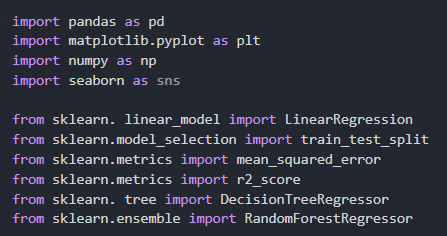
\includegraphics[width=0.75\textwidth]{../images/1-import.png}
    \caption{Perintah Install Library Seaborn}
    \label{1}
\end{figure}

\subsection{Load Dataset}
Pada praktikum ini, dataset yang digunakan adalah dataset harga rumah dengan link kaggle berikut \url{https://www.kaggle.com/datasets/shivachandel/kc-house-data}, atau praktikan juga dapat mengakses dataset secara langsung melalui repository yang telah disediakan. 

\begin{lstlisting}[language=Python, style=pythonnb]
df=pd.read_csv('https://raw.githubusercontent.com/ganjar87
/data_science_practice/main/kc_house_data.csv')    
\end{lstlisting}

\subsection{Exploratory Data Analysis (EDA)}
\subsubsection{Melihat 5 baris pertama dan terakhir}
\begin{figure}[H]
    \centering
    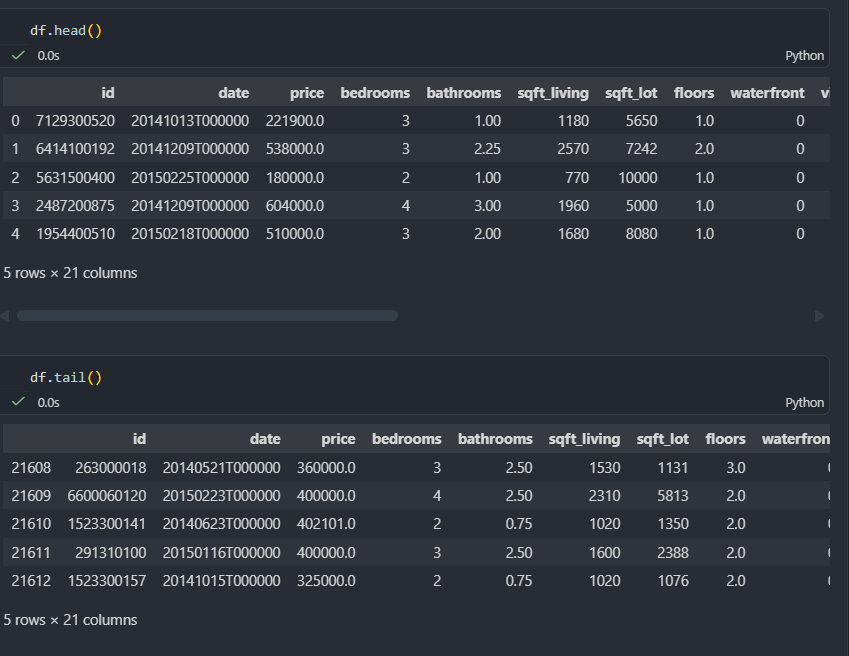
\includegraphics[width=0.85\textwidth]{../images/2-head-tail.png}
    \caption{Melihat 5 baris pertama dan terakhir}
    \label{2}
\end{figure}
\subsubsection{Melihat deskripsi statistik dengan df.describe()}
\begin{figure}[H]
    \centering
    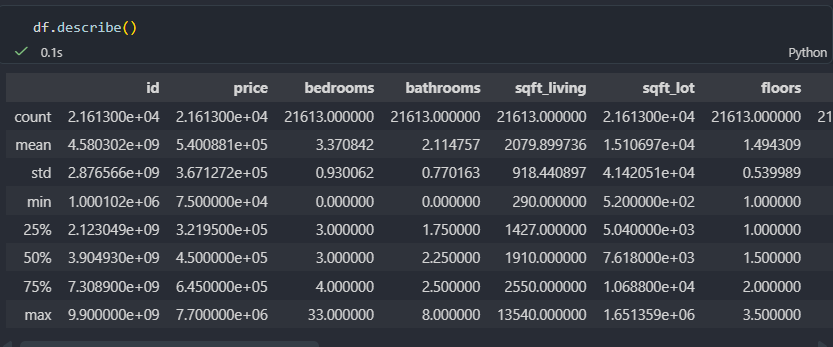
\includegraphics[width=0.85\textwidth]{../images/3-describe.png}
    \caption{Deskripsi Statistik}
    \label{3}
\end{figure}

\subsubsection{Melihat histogram}
\begin{figure}[H]
    \centering
    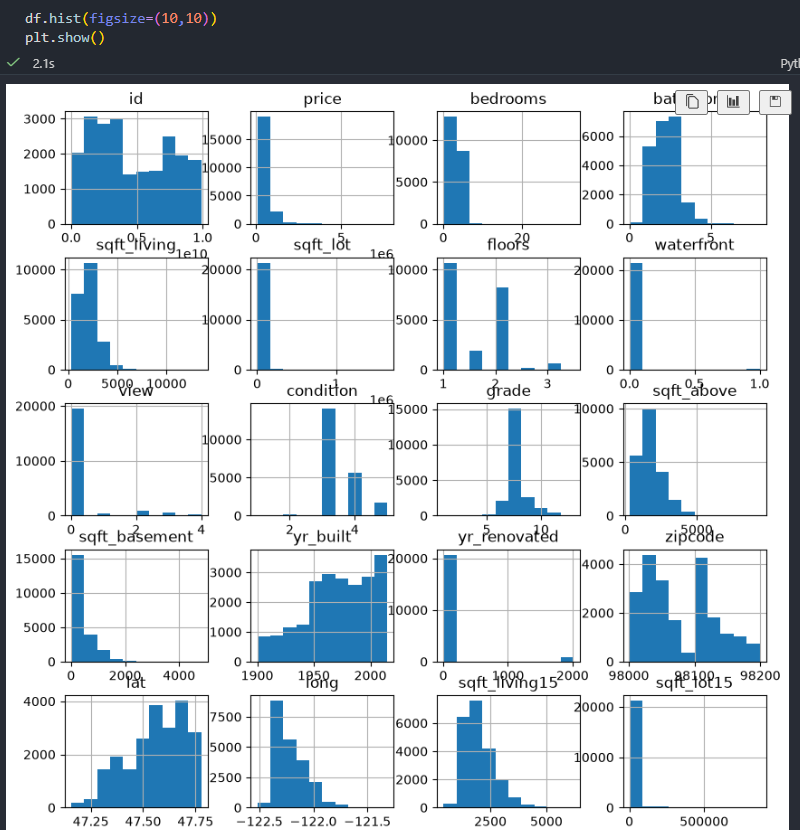
\includegraphics[width=0.85\textwidth]{../images/4-histogram.png}
    \caption{Histogram}
    \label{4}
\end{figure}

\subsubsection{Mengecek korelasi atribut numeric dengan df.corr(numeric\_only = True)}
\begin{figure}[H]
    \centering
    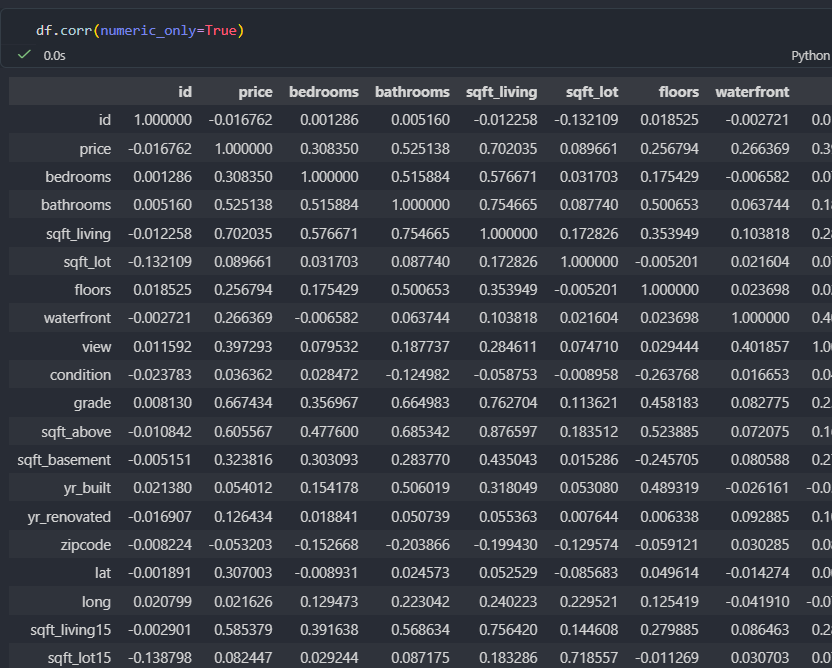
\includegraphics[width=0.85\textwidth]{../images/5-corr.png}
    \caption{Korelasi Atribut Numerik}
    \label{5}
\end{figure}

\subsubsection{Mengecek missing value dengan df.isnull().sum()}
\begin{figure}[H]
    \centering
    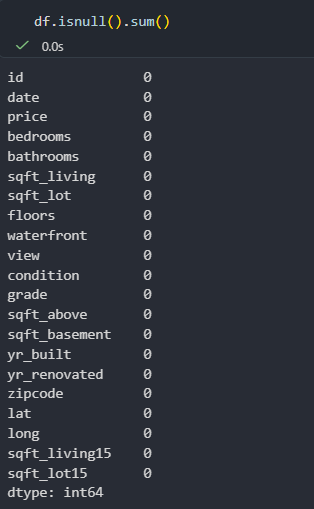
\includegraphics[width=0.55\textwidth]{../images/6-missing.png}
    \caption{Missing Value}
    \label{6}
\end{figure}
Dapat dilihat pada gambar \ref{6} bahwa tidak terdapat missing value pada dataset ini. Sehingga tidak perlu dilakukan penanganan missing value.

\subsubsection{Mengecek atribut kategorikal}
\begin{figure}[H]
    \centering
    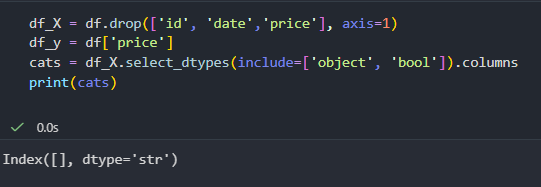
\includegraphics[width=0.85\textwidth]{../images/7-categorical.png}
    \caption{Atribut Kategorikal}
    \label{7}
\end{figure}

\subsection{Modelling}
\subsubsection{Linear Regression}
\begin{figure}[H]
    \centering
    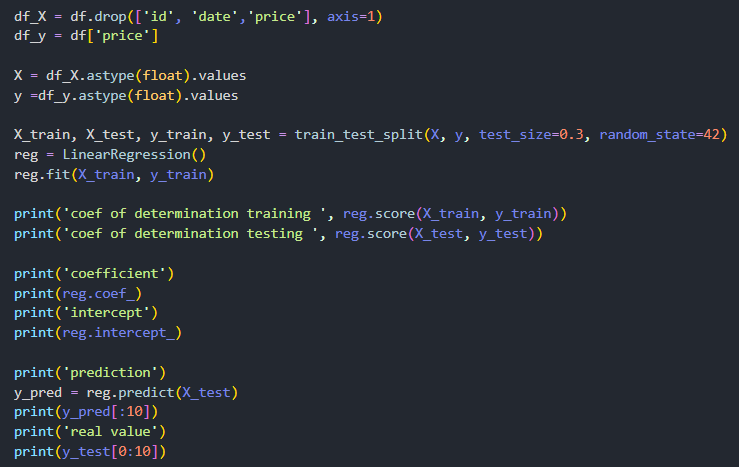
\includegraphics[width=0.95\textwidth]{../images/8-LR.png}
    \caption{Linear Regression}
    \label{8}
\end{figure}
Kode tersebut diawali dengan memisahkan variabel prediktor dan variabel target, yaitu menghapus kolom \texttt{id}, \texttt{date}, dan \texttt{price} dari fitur menggunakan \texttt{drop()}, sedangkan kolom \texttt{price} digunakan sebagai target. Data kemudian dikonversi menjadi tipe \texttt{float} dan \textit{NumPy array} agar dapat diproses oleh model. Selanjutnya, dataset dibagi menjadi data latih sebesar $70\%$ dan data uji sebesar $30\%$ menggunakan \texttt{train\_test\_split()} dengan \texttt{random\_state=42} agar pembagian data konsisten. Model \textit{Linear Regression} dibuat menggunakan \texttt{LinearRegression()} dan dilatih dengan data latih menggunakan \texttt{fit()}. Setelah pelatihan, metode \texttt{score()} digunakan untuk memperoleh nilai \textit{coefficient of determination} ($R^2$) pada data latih dan data uji. Atribut \texttt{coef\_} digunakan untuk memperoleh koefisien regresi, sedangkan \texttt{intercept\_} digunakan untuk memperoleh nilai konstanta model. Terakhir, metode \texttt{predict()} digunakan untuk menghasilkan prediksi harga berdasarkan data uji, kemudian hasil prediksi tersebut dibandingkan dengan nilai aktual yang tersimpan pada \texttt{y\_test}.

Outputnya dapat dilihat pada gambar \ref{output-lr}.
\begin{figure}[H]
    \centering
    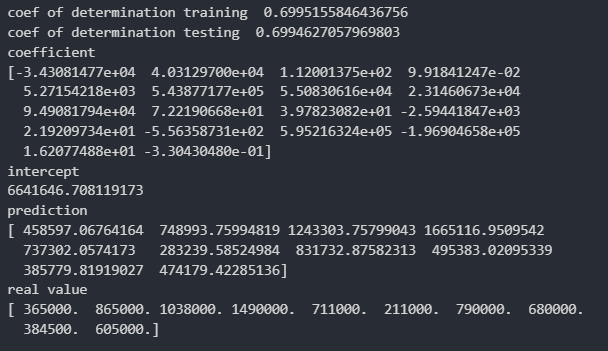
\includegraphics[width=0.85\textwidth]{../images/9-output-lr.png}
    \caption{Output Linear Regression}
    \label{output-lr}
\end{figure}

Tahap selanjutnya yaitu evaluasi model menggunakan RMSE dan $R^2$.
\begin{figure}[H]
    \centering
    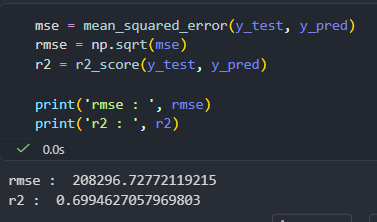
\includegraphics[width=0.85\textwidth]{../images/10-eval-lr.png}
    \caption{Evaluasi Model Linear Regression}
    \label{eval-lr}
\end{figure}
Kode tersebut digunakan untuk menghitung metrik evaluasi model regresi, yaitu \textit{Root Mean Squared Error} (RMSE) dan \textit{coefficient of determination} ($R^2$). Fungsi \texttt{mean\_squared\_error()} menghitung MSE berdasarkan nilai aktual \texttt{y\_test} dan hasil prediksi \texttt{y\_pred}, kemudian akar kuadratnya dihitung menggunakan \texttt{np.sqrt()} untuk memperoleh RMSE. Selanjutnya, fungsi \texttt{r2\_score()} digunakan untuk menghitung nilai $R^2$. Berdasarkan hasil pengujian, diperoleh nilai RMSE sebesar $208296.73$, yang menunjukkan rata-rata besarnya kesalahan prediksi model sekitar $208.297$ satuan nilai target. Sementara itu, nilai $R^2$ sebesar $0.69946$ menunjukkan bahwa model mampu menjelaskan sekitar $69.95\%$ variasi pada variabel target, sedangkan sekitar $30.05\%$ variasi lainnya belum dapat dijelaskan oleh model.

Tahap selanjutnya, dilakukan visualisasi untuk membandingkan antara nilai prediksi model dan nilai sebenarnya dari dataset testing.
\begin{figure}[H]
    \centering
    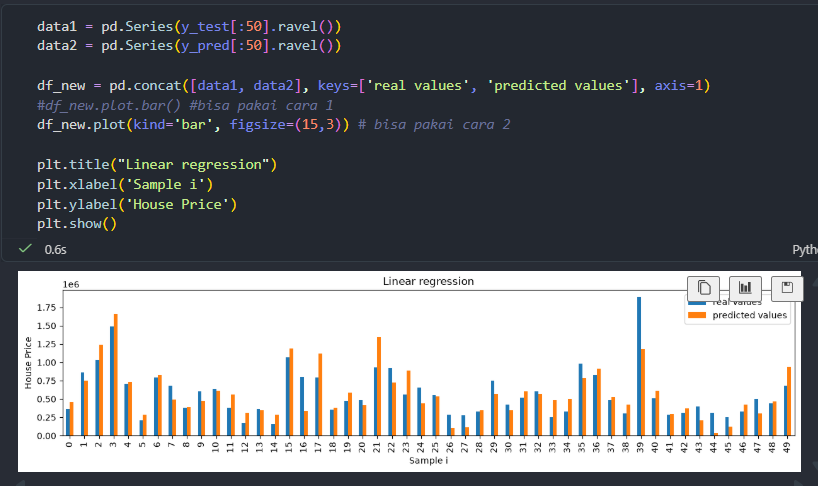
\includegraphics[width=0.95\textwidth]{../images/11-visual-lr.png}
    \caption{Visualisasi Prediksi vs Aktual Linear Regression}
    \label{visual-lr}
\end{figure}

\subsubsection{Decision Tree Regression}
\begin{figure}[H]
    \centering
    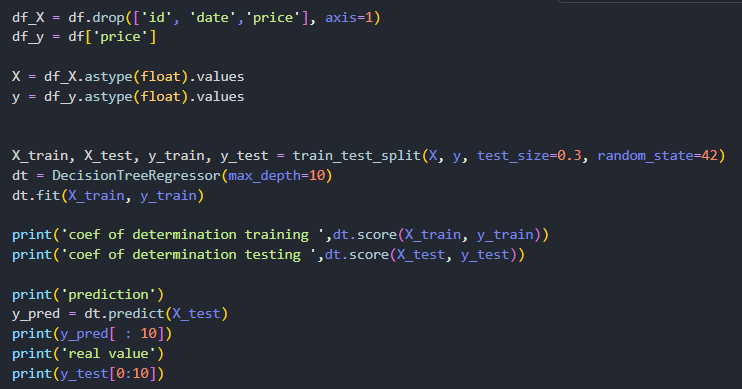
\includegraphics[width=0.95\textwidth]{../images/12-code-dtr.png}
    \caption{Decision Tree Regression}
    \label{12} 
\end{figure}
Kode tersebut digunakan untuk membangun model \textit{Decision Tree Regression} dalam memprediksi variabel \texttt{price}. Kolom \texttt{id}, \texttt{date}, dan \texttt{price} terlebih dahulu dihapus dari variabel prediktor, sedangkan \texttt{price} digunakan sebagai target. Data kemudian dikonversi menjadi tipe \texttt{float} dan dibagi menjadi data latih sebesar $70\%$ serta data uji sebesar $30\%$. Model \texttt{DecisionTreeRegressor} dibuat dengan parameter \texttt{max\_depth=10}, yang membatasi kedalaman maksimum pohon hingga 10 tingkat, kemudian dilatih menggunakan \texttt{fit()}. Selanjutnya, \texttt{score()} digunakan untuk menghitung nilai $R^2$ pada data latih dan data uji. Terakhir, \texttt{predict()} digunakan untuk menghasilkan prediksi pada data uji, yang kemudian dibandingkan dengan 10 nilai aktual pertama dari \texttt{y\_test}.

Outputnya dapat dilihat pada gambar \ref{output-dtr}.
\begin{figure}[H]
    \centering
    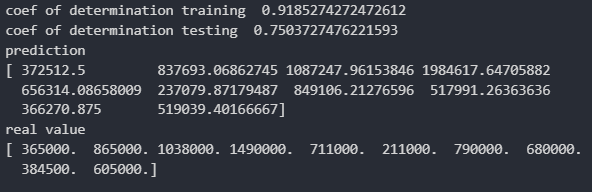
\includegraphics[width=0.85\textwidth]{../images/13-output-dtr.png}
    \caption{Output Decision Tree Regression}
    \label{output-dtr}
\end{figure}

Selanjutnya dilakukan evaluasi model menggunakan metrik RMSE dan $R^2$.
\begin{figure}[H]
    \centering
    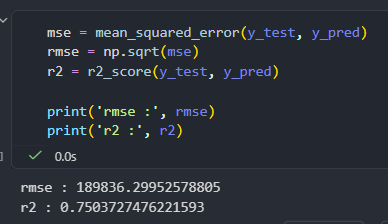
\includegraphics[width=0.75\textwidth]{../images/14-eval-dtr.png}
    \caption{Evaluasi Model Decision Tree Regression}
    \label{eval-dtr}
\end{figure}
Kode tersebut digunakan untuk mengevaluasi performa model \textit{Decision Tree Regression} menggunakan metrik RMSE dan $R^2$. Fungsi \texttt{mean\_squared\_error()} menghitung nilai MSE antara nilai aktual \texttt{y\_test} dan nilai prediksi \texttt{y\_pred}, kemudian \texttt{np.sqrt()} digunakan untuk memperoleh nilai RMSE. Selanjutnya, fungsi \texttt{r2\_score()} menghitung nilai \textit{coefficient of determination} ($R^2$). Berdasarkan output, diperoleh nilai RMSE sebesar $189836.30$, yang menunjukkan bahwa rata-rata besarnya kesalahan prediksi model sekitar $189.836$ satuan nilai target. Nilai $R^2$ sebesar $0.75037$ menunjukkan bahwa model mampu menjelaskan sekitar $75.04\%$ variasi pada variabel target, sedangkan sekitar $24.96\%$ variasi lainnya belum dapat dijelaskan oleh model. Dibandingkan hasil Linear Regression sebelumnya, model Decision Tree menghasilkan RMSE yang lebih rendah dan $R^2$ yang lebih tinggi, sehingga pada data pengujian tersebut Decision Tree memiliki performa prediksi yang lebih baik.

Tahap selanjutnya, dilakukan visualisasi untuk membandingkan antara nilai prediksi model dan nilai sebenarnya dari dataset testing. 
\begin{figure}[H]
    \centering
    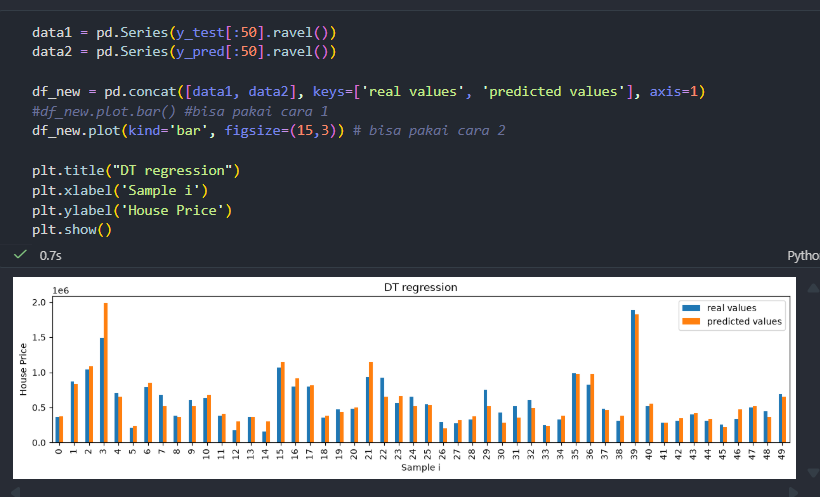
\includegraphics[width=0.95\textwidth]{../images/15-visual-dtr.png}
    \caption{Visualisasi Prediksi vs Aktual Decision Tree Regression}
    \label{visual-dtr}
\end{figure}

\subsubsection{Random Forest Regression}
\begin{figure}[H]
    \centering
    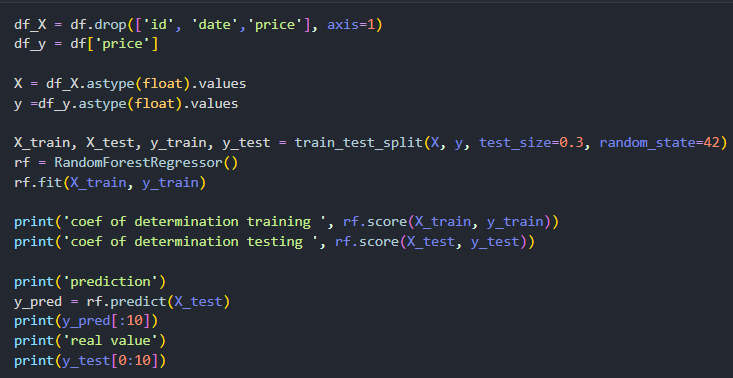
\includegraphics[width=0.95\textwidth]{../images/16-code-rfr.png}
    \caption{Random Forest Regression}
    \label{16}
\end{figure}
Kode tersebut digunakan untuk membangun model \textit{Random Forest Regression} dalam memprediksi variabel \texttt{price}. Kolom \texttt{id}, \texttt{date}, dan \texttt{price} terlebih dahulu dihapus dari variabel prediktor, sedangkan \texttt{price} digunakan sebagai variabel target. Data kemudian dikonversi menjadi tipe \texttt{float} dan dibagi menjadi data latih sebesar $70\%$ serta data uji sebesar $30\%$ menggunakan \texttt{train\_test\_split()} dengan \texttt{random\_state=42}. Model \texttt{RandomForestRegressor()} dibuat untuk membangun sejumlah pohon keputusan dan menggabungkan hasil prediksinya, kemudian dilatih menggunakan \texttt{fit()}. Selanjutnya, \texttt{score()} digunakan untuk menghitung nilai \textit{coefficient of determination} ($R^2$) pada data latih dan data uji. Terakhir, metode \texttt{predict()} digunakan untuk menghasilkan prediksi harga berdasarkan data uji, yang kemudian dibandingkan dengan 10 nilai aktual pertama dari \texttt{y\_test}.

Outputnya dapat dilihat pada gambar \ref{output-rfr}.
\begin{figure}[H]
    \centering
    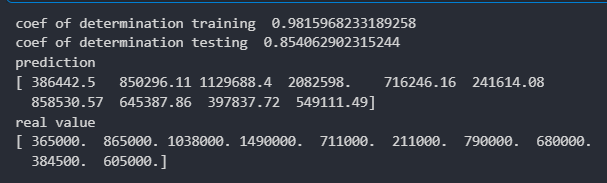
\includegraphics[width=0.85\textwidth]{../images/17-output-rfr.png}
    \caption{Output Random Forest Regression}
    \label{output-rfr}
\end{figure}    

Selanjutnya dilakukan evaluasi model menggunakan metrik RMSE dan $R^2$.
\begin{figure}[H]
    \centering
    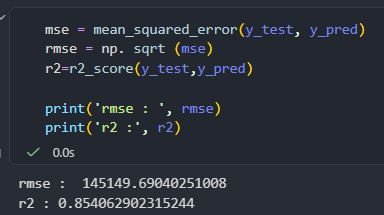
\includegraphics[width=0.75\textwidth]{../images/18-eval-rfr.png}
    \caption{Evaluasi Model Random Forest Regression}
    \label{eval-rfr}
\end{figure}
Kode tersebut digunakan untuk mengevaluasi performa model \textit{Random Forest Regression} menggunakan metrik RMSE dan $R^2$. Fungsi \texttt{mean\_squared\_error()} menghitung nilai MSE antara nilai aktual dan prediksi, kemudian \texttt{np.sqrt()} digunakan untuk memperoleh nilai RMSE. Selanjutnya, \texttt{r2\_score()} menghitung nilai \textit{coefficient of determination} ($R^2$). Berdasarkan output, diperoleh RMSE sebesar $145149.69$, yang menunjukkan rata-rata kesalahan prediksi sekitar $145.150$ satuan nilai target. Nilai $R^2$ sebesar $0.85406$ menunjukkan bahwa model mampu menjelaskan sekitar $85.41\%$ variasi pada variabel target, sedangkan sekitar $14.59\%$ sisanya belum dapat dijelaskan oleh model. Hasil tersebut menunjukkan performa Random Forest yang lebih baik dibandingkan Linear Regression dan Decision Tree berdasarkan nilai RMSE yang lebih rendah dan $R^2$ yang lebih tinggi.

Selanjutnya, dilakukan visualisasi untuk membandingkan antara nilai prediksi model dan nilai sebenarnya dari dataset testing.
\begin{figure}[H]
    \centering
    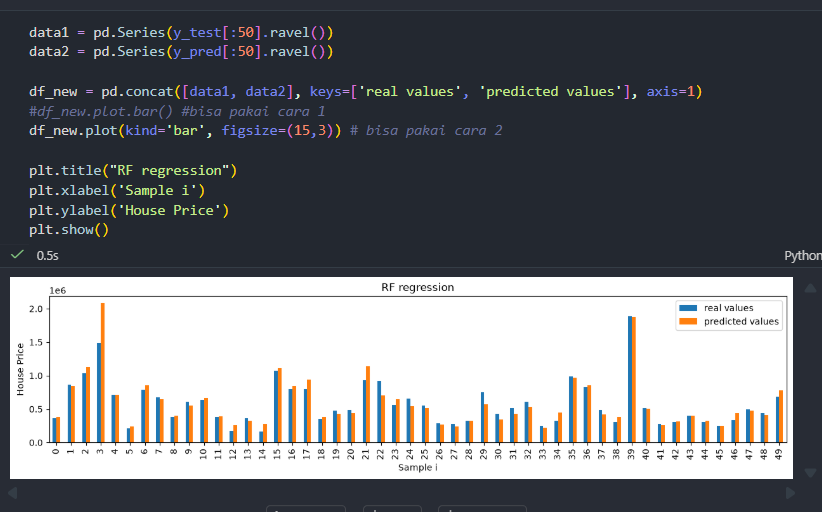
\includegraphics[width=0.95\textwidth]{../images/19-visualisasi-rfr.png}
    \caption{Visualisasi Prediksi vs Aktual Random Forest Regression}
    \label{visual-rfr}
\end{figure}
Visualisasi tersebut membandingkan nilai aktual (\textit{real values}) dengan nilai hasil prediksi (\textit{predicted values}) dari model \textit{Random Forest Regression} pada 50 sampel data uji. Sumbu-$x$ menunjukkan nomor sampel, sedangkan sumbu-$y$ menunjukkan nilai \textit{House Price}. Batang yang berdekatan menunjukkan perbandingan antara harga aktual dan harga yang diprediksi oleh model. Secara umum, sebagian besar batang prediksi memiliki nilai yang relatif dekat dengan nilai aktual, meskipun terdapat beberapa perbedaan yang cukup besar, seperti pada sampel ke-3. Kedekatan antara kedua batang menunjukkan bahwa model mampu menghasilkan prediksi yang cukup mendekati nilai sebenarnya, yang sejalan dengan hasil evaluasi sebelumnya berupa nilai RMSE sebesar $145149.69$ dan $R^2$ sebesar $0.85406$.

\section{Tugas dan Analisis}
\subsection{Tujuan Penggunaan Dataset}
Diberikan dataset dengan link berikut \url{https://www.kaggle.com/datasets/hellbuoy/car-price-prediction/data}.

\begin{figure}[H]
    \centering
    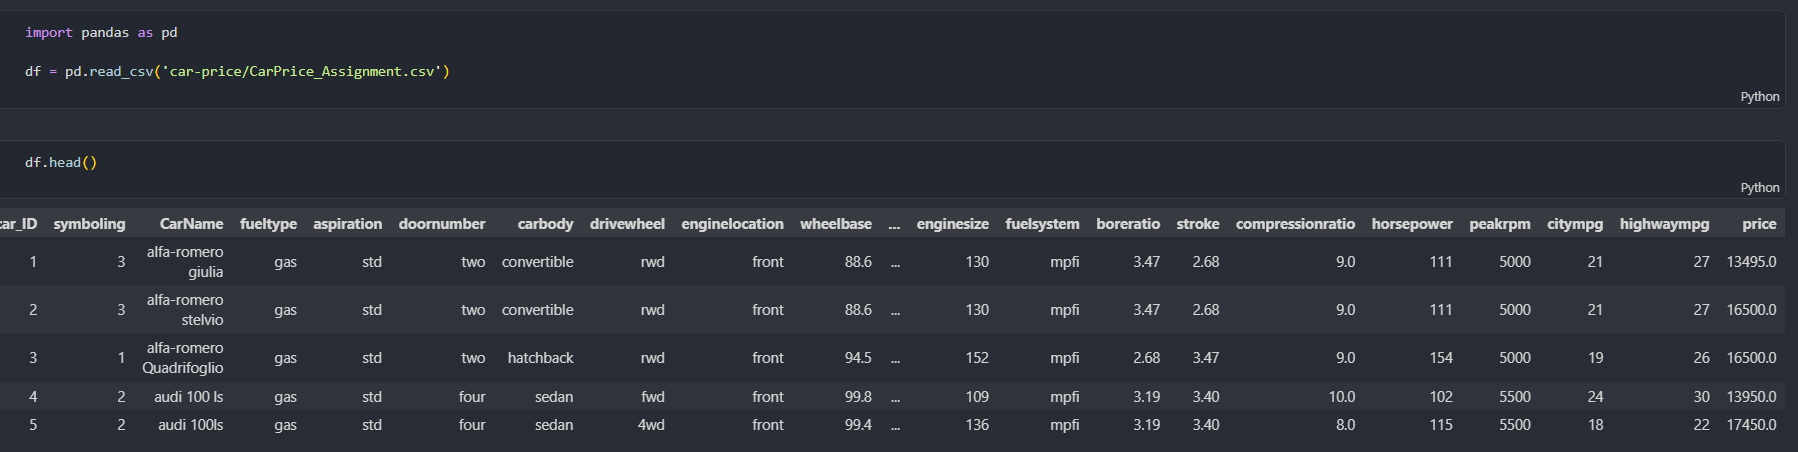
\includegraphics[width=0.95\textwidth]{../images/20-dataset-car-price.png}
    \caption{Dataset Car Price Prediction}
    \label{dataset-car-price}
\end{figure}

Dataset Car Price Prediction digunakan untuk menganalisis faktor-faktor yang memengaruhi harga sebuah mobil serta membangun model machine learning yang dapat memprediksi harga mobil berdasarkan karakteristiknya. Dataset terdiri dari berbagai atribut kendaraan seperti ukuran kendaraan, berat kendaraan, jenis mesin, kapasitas mesin, horsepower, konsumsi bahan bakar, dan atribut kategorikal lainnya. Target atau output yang digunakan adalah atribut price, sedangkan atribut lainnya digunakan sebagai input atau variabel independen. car\_ID tidak digunakan karena hanya merupakan identitas unik data, sedangkan CarName tidak digunakan dalam eksperimen ini karena memiliki banyak kategori unik.

\subsection{Variabel yang paling mempengaruhi output}
\begin{figure}[H]
    \centering
    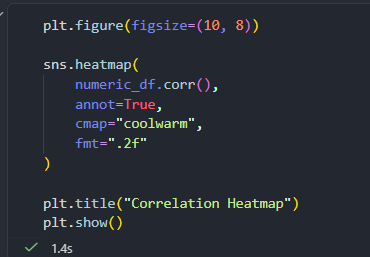
\includegraphics[width=0.75\textwidth]{../images/21-corr-car-price.png}
    \caption{Korelasi Atribut Numerik Dataset Car Price Prediction}
    \label{corr-car-price}
\end{figure}

\begin{figure}[H]
    \centering
    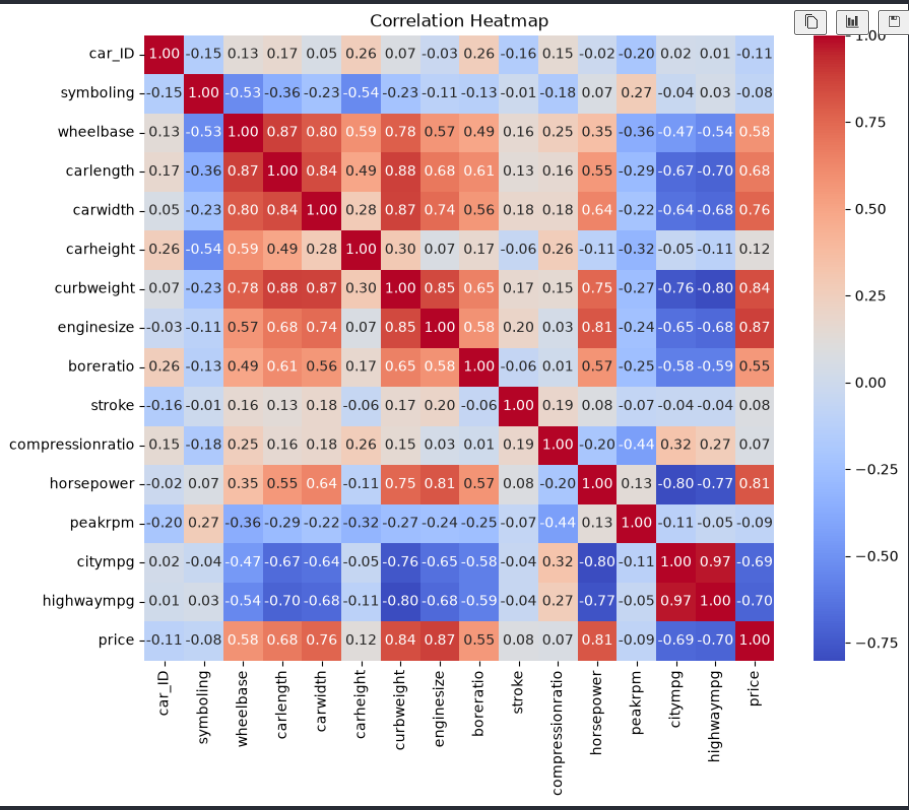
\includegraphics[width=0.95\textwidth]{../images/22-visualisasi-corr.png}
    \caption{Heatmap Korelasi Atribut Numerik Dataset Car Price Prediction}
    \label{corr-car-price-heatmap}
\end{figure}

\begin{figure}[H]
    \centering
    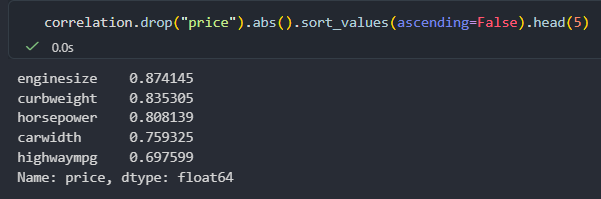
\includegraphics[width=0.95\textwidth]{../images/23-corr-data.png}
    \caption{Visualisasi Korelasi Atribut Numerik Dataset Car Price Prediction}
    \label{corr-car-price-visual}
\end{figure}
Dapat dilihat pada heatmap korelasi pada gambar \ref{corr-car-price-visual} bahwa Output tersebut menunjukkan lima variabel yang memiliki nilai korelasi absolut tertinggi terhadap variabel \texttt{price}. Variabel \texttt{enginesize} memiliki korelasi sebesar $0.874145$, diikuti oleh \texttt{curbweight} sebesar $0.835305$, \texttt{horsepower} sebesar $0.808139$, \texttt{carwidth} sebesar $0.759325$, dan \texttt{highwaympg} sebesar $0.697599$. Karena seluruh nilai korelasi bernilai positif, kelima variabel tersebut memiliki hubungan positif dengan harga mobil. Variabel \texttt{enginesize} memiliki korelasi paling tinggi, sehingga dapat dikatakan sebagai variabel yang memiliki hubungan paling kuat dengan \texttt{price} dibandingkan variabel lainnya pada hasil tersebut.


\subsection{Model Regresi}
\subsubsection{Linear Regression}
\begin{figure}[H]
    \centering
    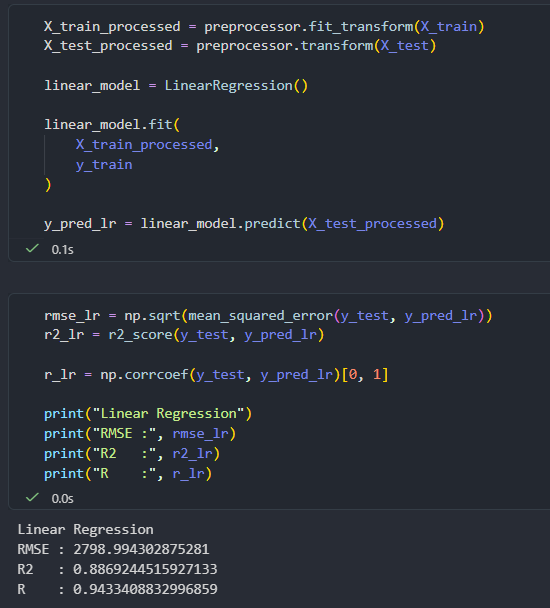
\includegraphics[width=0.95\textwidth]{../images/25-lr.png}
    \caption{Linear Regression}
    \label{linear-regression}
\end{figure}

\subsubsection{Decision Tree Regression}
\begin{figure}[H]
    \centering
    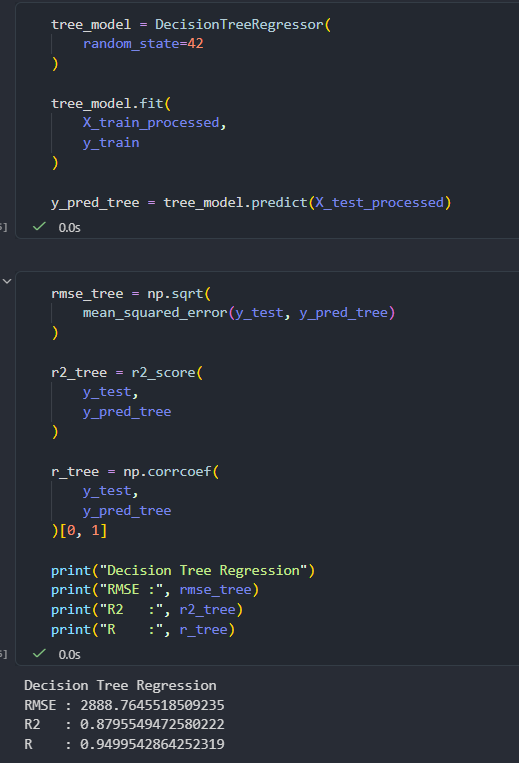
\includegraphics[width=0.95\textwidth]{../images/26-dtr.png}
    \caption{Decision Tree Regression}
    \label{decision-tree-regression}
\end{figure}

\subsubsection{Random Forest Regression}
\begin{figure}[H]
    \centering
    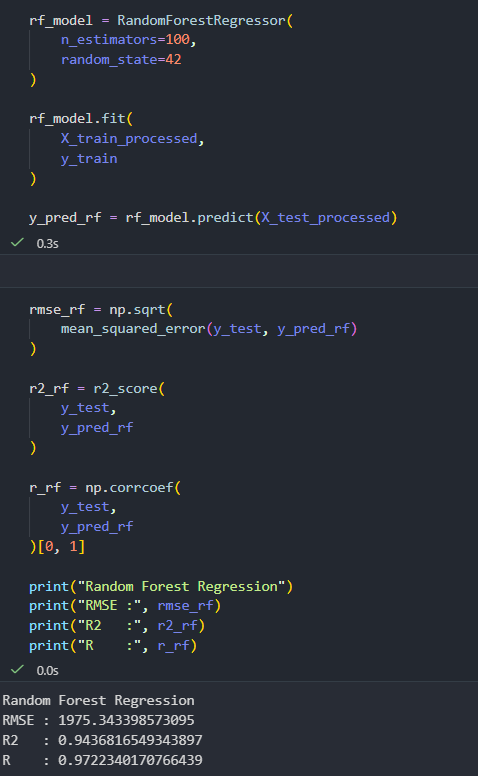
\includegraphics[width=0.95\textwidth]{../images/27-rfr.png}
    \caption{Random Forest Regression}
    \label{random-forest-regression}
\end{figure}

\subsection{Perbandingan performa Model}
\begin{figure}[H]
    \centering
    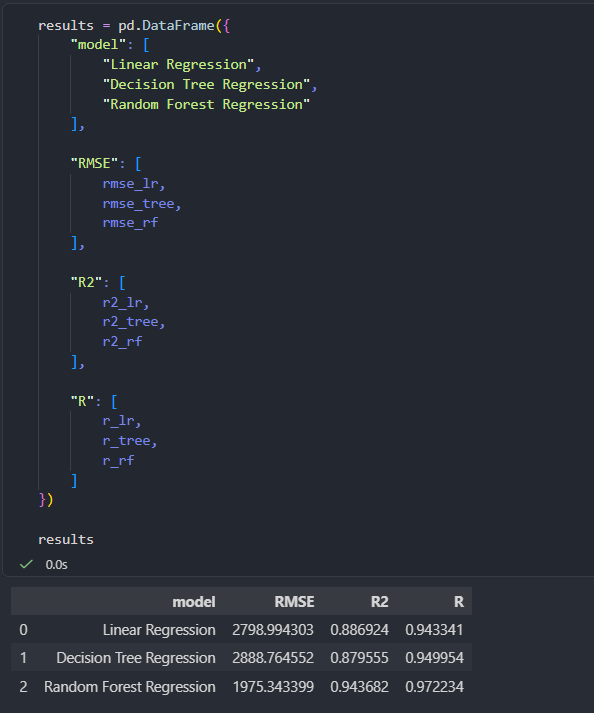
\includegraphics[width=0.95\textwidth]{../images/24-tabel-evaluasi.png}
    \caption{Perbandingan Performa Model}
    \label{perbandingan-model}
\end{figure}
Output tersebut menunjukkan perbandingan performa tiga model regresi berdasarkan metrik RMSE, $R^2$, dan koefisien korelasi ($R$). \textit{Random Forest Regression} memiliki performa terbaik dengan RMSE sebesar $1975.34$, $R^2$ sebesar $0.943682$, dan $R$ sebesar $0.972234$. Sementara itu, \textit{Linear Regression} memperoleh RMSE $2798.99$ dan $R^2$ $0.886924$, sedangkan \textit{Decision Tree Regression} memperoleh RMSE $2888.76$ dan $R^2$ $0.879555$. Dengan demikian, \textit{Random Forest Regression} merupakan model terbaik karena memiliki nilai RMSE paling rendah serta nilai $R^2$ dan $R$ paling tinggi dibandingkan kedua model lainnya.

\subsection{Hasil Eksperimen}
Berdasarkan hasil eksperimen, Random Forest Regression merupakan model dengan performa terbaik dibandingkan Linear Regression dan Decision Tree Regression. Hal tersebut ditunjukkan oleh nilai RMSE yang paling rendah serta nilai R² dan R yang paling tinggi. RMSE yang rendah menunjukkan bahwa kesalahan prediksi harga relatif kecil, sedangkan nilai R² yang tinggi menunjukkan bahwa model mampu menjelaskan variasi harga dengan lebih baik. Random Forest juga terdiri dari banyak Decision Tree sehingga mampu menangkap hubungan non-linear antara karakteristik kendaraan dan harga dengan lebih baik dibandingkan Linear Regression yang hanya memodelkan hubungan linear dan satu Decision Tree yang lebih rentan terhadap overfitting.

\newpage
\section{Kesimpulan}
Berdasarkan praktikum yang telah dilakukan, dapat disimpulkan bahwa model Random Forest Regression memiliki performa terbaik dibandingkan Linear Regression dan Decision Tree Regression. Hal ini ditunjukkan oleh nilai RMSE yang lebih rendah dan nilai $R^2$ yang lebih tinggi pada data uji. Model Random Forest mampu menangkap hubungan non-linear dan interaksi antarvariabel dengan lebih baik, sehingga menghasilkan prediksi yang lebih akurat terhadap harga rumah.

Berdasarkan hasil eksperimen, pemilihan model regresi sebaiknya mempertimbangkan karakteristik data, kompleksitas hubungan antarvariabel, serta kebutuhan interpretasi model. Random Forest Regression dapat menjadi pilihan yang baik ketika performa prediksi menjadi prioritas utama, meskipun memiliki kompleksitas yang lebih tinggi dibandingkan Linear Regression dan Decision Tree Regression.

\newpage
\renewcommand{\refname}{\section{Daftar Pustaka}}
\bibliographystyle{IEEEtran}
\bibliography{ref}
\end{document}
